%!TEX root = ../thesis.tex
\chapter{Validation}
\label{chap:validation}

The main goal of this thesis was to develop a solution for bridging the gap between the simulation and MAS domains that, while maintaining a familiar JADE-like environment, would offer significant performance improvements to MABS development. To validate this approach and the developed tools, a set of experiments were designed, in an attempt to cover and test all the available features.

The first example consists in a simple contract net between one buyer and multiple sellers. In the second example, multiple contract nets run concurrently and some of the buyers include available computational trust about sellers. The third example is a board game called Risk developed prior to this thesis. The goal of this last example was to test SAJaS in a ``real'' example of an already developed MAS, one that had not been developed specifically for this thesis. All tests were performed in a laptop using an Intel i7 CPU (8 logical cores) at 2.20 GHz and 8GB of RAM.

%!TEX root = ../thesis.tex
\section{Simple Contract Net}

In this scenario, one agent sends a call for proposals (CFP) to multiple agents which then reply with their individual proposals. This simple scenario was created to test the core of SAJaS and the plugin. The goal was not only to create a working simulation model based on SAJaS, but also to demonstrate that the execution of a simulation in SAJaS and the equivalent JADE application generated from it are identical and that performance in SAJaS is higher.

\subsection{Experimental Setup}

The diagram in Figure \ref{fig:CNetExample} illustrates the contract net created for this test. An agent (the buyer) intends to purchase a certain quantity of three kinds of goods: rice, flour and oats. Besides the quantities of each product it needs, the buyer also stipulates a maximum price for the whole deal. The buyer will issue a call for proposals (CFP) containing a request for supplies to all agents that announce themselves as suppliers in the DF.

Supplier agents have a maximum supply capacity and a price for each product. After receiving a CFP, the supplier replies with a PROPOSAL containing a price for each product if the demanded supply is within the seller's capacity. Otherwise, a REFUSE message will be sent to the buyer.
Finally, the buyer agent compares all valid proposals, chooses the cheapest offer for each of the three products and replies with an ACCEPT PROPOSAL to the best offers, and REJECT PROPOSAL to all others.

\begin{figure}[h]
	\centering
	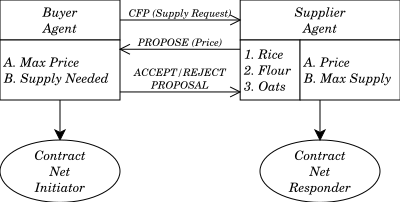
\includegraphics[width=0.60\linewidth]{figures/CNetExample.pdf}
	\caption{Representation of the contract net scenario.}
	\label{fig:CNetExample}
\end{figure}

To ensure the proper comparison of results, a fixed data set with values for prices and demand was used in both frameworks. This experiment focused on two simple metrics to evaluate the result: time and outcome. 

Multiple executions were performed with varying numbers of suppliers (as sugested by Figure \ref{fig:performance}); for each case, the simulation was executed 10 times. The execution time was measured from be begining of the protocol, until all suppliers were notified.

In JADE, the simulation was tested in two different setups: first, with all agents running in a single container; second, with the supplier agents in one container and the buyer in a separate one (but in the same host). In this configuration, all communication between agents happens across containers. The second validation metric was the actual result of the protocol, i.e who were the supplier agents chosen by the buyer and their price proposals.

\subsection{Results}

For each number of agents, the experiment was run 10 times. The average performance of of the experiment for each number of agents is represented in Figure \ref{fig:performance}. The performance of the simulation based on SAJaS was significantly better, excelling when the number of agents is high. JADE was able to perform better when using two distinct containers. JADE's performance drops very significantly when there is a high communication-to-computation ratio in the application. Also, JADE is capable of performing some optimizations when two interacting agents are located within the same containers\cite{mengistu2008scalability}.

Regarding the outcome of the protocol, the same values were obtained in both implementations for each number of agents, confirming that the execution is identical in both implementations.

\begin{figure}[h]
	\centering
	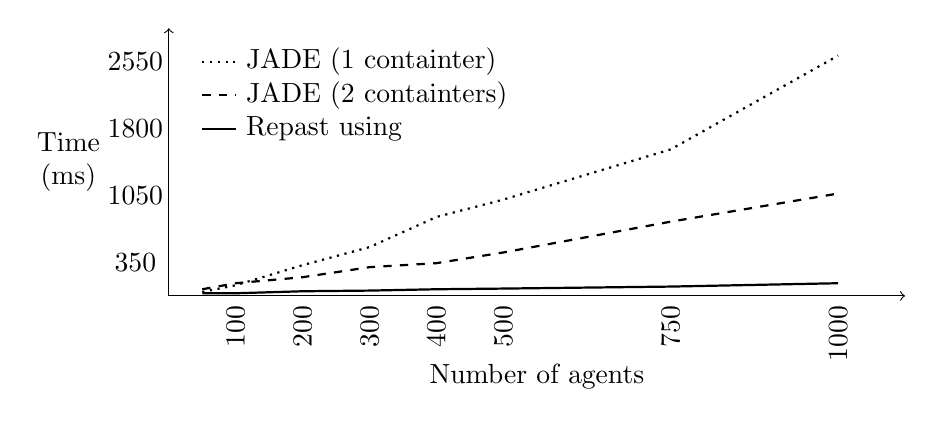
\begin{tikzpicture}[scale=0.85]

		% horizontal axis
		\draw[->] (0,0) -- (11,0);
		\draw (5.5,-1.2) node[align=center] {Number of agents}; %label

		
		% labels
		\draw	%(0.5,0) node[rotate=90, anchor=east] {50}
				(1.0,0) node[rotate=90, anchor=east] {100}
				(2.0,0) node[rotate=90, anchor=east] {200}
				(3.0,0) node[rotate=90, anchor=east] {300}
				(4.0,0) node[rotate=90, anchor=east] {400}
				(5.0,0) node[rotate=90, anchor=east] {500}
				(7.5,0) node[rotate=90, anchor=east] {750}
				(10.,0) node[rotate=90, anchor=east] {1000};

		\draw	(-0.5,0.5) node[anchor=center] {350}
				(-0.5,1.5) node[anchor=center] {1050}
				(-0.5,2.5) node[anchor=center] {1800}
				(-0.5,3.5) node[anchor=center] {2550};
		% vertical axis
		\draw[->] (0,0) -- (0,4);
		\draw (-1.5,2) node[align=center] {Time\\(ms)}; %label
		%\draw (-1.5,1.6) node[align=center] {(ms)}; %label

		%% Data %%
		% JADE 2 containers
		\draw[thick,dashed] (0.5,3.0) --
			(1,3.0) node[anchor=west, pos=1.0] {JADE (2 containters)}; %subtitle
		\draw[thick,dashed] (0.5, 0.10) --
					(1.0, 0.19) --
					(2.0, 0.28) --
					(3.0, 0.43) --
					(4.0, 0.49) --
					(5.0, 0.65) --
					(7.5, 1.11) --
					(10., 1.53);
		% JADE 1 containers
		\draw[thick,dotted] (0.5,3.5) --
			(1,3.5) node[anchor=west, pos=1.0] {JADE (1 containter)}; %subtitle
		\draw[thick,dotted] (0.5, 0.06) --
					(1.0, 0.16) --
					(2.0, 0.46) --
					(3.0, 0.73) --
					(4.0, 1.18) --
					(5.0, 1.44) --
					(7.5, 2.19) --
					(10., 3.59);
		% Repast
		\draw[thick] (0.5,2.5) --
			(1,2.5) node[anchor=west, pos=1.0] {Repast using \apiname{}}; %subtitle
		\draw[thick] (0.5, 0.04) --
					(1.0, 0.04) --
					(2.0, 0.07) --
					(3.0, 0.08) --
					(4.0, 0.10) --
					(5.0, 0.11) --
					(7.5, 0.14) --
					(10., 0.19);


	\end{tikzpicture}
	\caption[Execution performance in a simple contract net]
	{Average execution time of each framework in the different experiments.}
	\label{fig:performance}
\end{figure}

%!TEX root = ../thesis.tex
\section{Multiple Contract Net using Trust}

This scenario is similar to the previous one, but attempts to perform a better coverage of the features present in SAJaS, namely the use of the AchieveRE Protocol and the Responder Dispatcher which allows for multiple contract nets to be handled without deadlocks occuring. However. rather than comparing the exact value obtained from the simulation as in the previous scenario, the goal is to compare the overall behaviour of all agents.

\subsection{Experimental Setup}
This simulation is composed by multiple buyers and multiple sellers running simultaneously. After the sellers register themselves in the DF, each buyer will perform a search for sellers of the particular good it needs to purchase. Then, the buyer sends this list of agents to the CTAgent (CT standing for computational trust). The CTAgent will calculate a trust value for each seller based on its past contracts with buyers and return the top 5 sellers.

With this information, the buyer sends a CFP only to the 5 top agents and accept the best proposal from them. Some sellers will occasionally violate the contract after acceptance. The buyer will then inform the CTAgent if the contract was fulfilled or violated. The compilation of this composes the trust of the seller.

Some buyers are programmed to ignore trust and rely solely on the proposal. The idea is that informed buyers eventually avoid contacting sellers programmed to violate contracts more often. The goal of this experiment is to model this scenario in SAJaS, convert it to JADE and verify that the obtained results are very similar.

After one contract is concluded, Buyers start a new one, performing a new DF search for the next product they want to buy, request information from the CTAgent and issuing a new CFP.

\subsection{Results}

The experiment was executed 5 times in JADE and 5 times in SAJaS. The scenario is composed of 20 buyers using computational trust, 20 not using trust and 80 sellers. A total of 2000 contracts were recorded to create the following charts in Figures \ref{fig:enterprise_JADE} and \ref{fig:enterprise_SAJaS}. As shown, buyers who made use of computational trust had more successful contracts. The fluctuations early in the simulation are due to the initial lack of trust information.

As expected and as shown in the charts, the same outcome was observed both in JADE and SAJaS. With this experiment, it was possible to test the Request protocol - when requesting computational trust, the Contract Net - when purchasing goods, the Responder Dispatcher - to handle CFPs from multiple buyers concurrently, the messaging system and the DF service.

In terms of performance, the outcome of this experiment, as ilustrated by the chart in Figure \ref{fig:enterprise_times}, may not seem as impressive when compared with the first experience. However, the algorithm employed to calculate trust is very time consuming. In a setup without the use of trust by any of the buyers, the performance difference between JADE and SAJaS is comparable to the first scenario.

\begin{figure}[ht]
	\centering
	\begin{subfigure}[b]{\textwidth}
		\centering
		\begin{tikzpicture}[scale=0.85]

			% horizontal axis
			\draw[->] (0,0) -- (11,0);
			\draw (5.5,-1.2) node[align=center] {Number of Contracts}; %label

			% labels
			\draw	(0  ,0) node[anchor=north] {0}
					(2.5,0) node[anchor=north] {500}
					(5  ,0) node[anchor=north] {1000}
					(7.5,0) node[anchor=north] {1500}
					(10 ,0) node[anchor=north] {2000};
			
			
			% vertical axis
			\draw[->] (0,0) -- (0,5);
			\draw (-1.1,2.5) node[rotate=90, anchor=south, align=center]
				{\% of Fullfielment}; %label
			\draw	(0, 1) node[anchor=east] {0.25}
					(0, 2) node[anchor=east] {0.50}
					(0, 3) node[anchor=east] {0.75}
					(0, 4) node[anchor=east] {1.00};
			
			

			%% Data %%

			%subtitles
			\draw[thick] (0.5,3.5) --
				(1,3.5) node[anchor=west, pos=1.0] {Using trust and proposal};
			\draw[thick, dotted]
				(0.5,4.5) --
				(1,4.5) node[anchor=west, pos=1.0] {Using only the proposal}; 

			%lines
			\input{chapters/charts/enterprise_values_jade}


		\end{tikzpicture}
		\caption{In SAJaS}
		\label{fig:enterprise_JADE}
	\end{subfigure}
	\bigskip\\
	\begin{subfigure}[b]{\textwidth}
		\centering
		\begin{tikzpicture}[scale=0.85]

			% horizontal axis
			\draw[->] (0,0) -- (11,0);
			\draw (5.5,-1.2) node[align=center] {Number of Contracts}; %label

			% labels
			\draw	(0  ,0) node[anchor=north] {0}
					(2.5,0) node[anchor=north] {500}
					(5  ,0) node[anchor=north] {1000}
					(7.5,0) node[anchor=north] {1500}
					(10 ,0) node[anchor=north] {2000};
			
			
			% vertical axis
			\draw[->] (0,0) -- (0,5);
			\draw (-1.1,2.5) node[rotate=90, anchor=south, align=center]
				{\% of Fullfielment}; %label
			\draw	(0, 1) node[anchor=east] {0.25}
					(0, 2) node[anchor=east] {0.50}
					(0, 3) node[anchor=east] {0.75}
					(0, 4) node[anchor=east] {1.00};

			%% Data %%

			%subtitles
			\draw[thick] (0.5,3.5) --
				(1,3.5) node[anchor=west, pos=1.0] {Using trust and proposal};
			\draw[thick, dotted] 
				(0.5,4.5) --
				(1,4.5) node[anchor=west, pos=1.0] {Using only the proposal}; 
			
			%lines
			\input{chapters/charts/enterprise_values_sajas}


		\end{tikzpicture}
		\caption{In JADE}
		\label{fig:enterprise_SAJaS}
	\end{subfigure}
	\caption[Multiple Contract Net scenario results in JADE]
	{Average result of 5 executions of the Multiple Contract Net scenario during 2000 contracts}
\end{figure}

\begin{figure}
	\centering
	\begin{tikzpicture}[scale=0.85]

		% horizontal axis
		\draw[->] (0,0) -- (11,0);
		\draw (5.5,-1.2) node[align=center] {Time/s}; %label

		% labels
		\draw	(1.4,0) node[anchor=north] {2}
				(2.8,0) node[anchor=north] {4}
				(4.2,0) node[anchor=north] {6}
				(5.6,0) node[anchor=north] {8}
				(7.1,0) node[anchor=north] {10}
				(8.5,0) node[anchor=north] {12}
				(9.9,0) node[anchor=north] {14};
		
		
		% vertical axis
		\draw[->] (0,0) -- (0,5);
		\draw (-1.1,2.5) node[rotate=90, anchor=south, align=center]
			{Number of Contracts}; %label
		\draw	(0, 0) node[anchor=north] {0}
				(0, 1) node[anchor=east] {500}
				(0, 2) node[anchor=east] {1000}
				(0, 3) node[anchor=east] {1500}
				(0, 4) node[anchor=east] {2000};
		
		

		%% Data 
		%subtitle
		\draw[thick] (0.5,3.5) --
			(1,3.5) node[anchor=west, pos=1.0] {SAJaS};
		%line
		\input{chapters/charts/enterprise_times}

		\draw[thick, dotted]%subtitle
			(0.5,4.5) --
			(1,4.5) node[anchor=west, pos=1.0] {JADE}; 


	\end{tikzpicture}
	\caption[Multiple Contract Net scenario results in Repast]
	{Number of contracts executed in JADE and SAJaS. Final number of contracts is 2000 for both frameworks.}
	\label{fig:enterprise_times}
\end{figure}

\input{chapters/validation:risk}


\section{Summary}

These three experiments were designed to validate the results of this thesis.Technically, the scenarios described in this chapter covered all currently available features in SAJaS. The Achieve RE protocol was used in the Enterprise scenario to communicate with the CT Agent and it was widely used in Risk for all communications. The Contract Net protocol was covered in the first two experiments. The Enterprise scenario also allowed multiple concurrent contracts to take place by using the Responder Dispatcher.

All scenarios made use of the DF service, the AMS, the MTS and of containers like the ACL Message, the Message Template, the DFAgentDescription and the Service Description. The creation of custom Simple Behaviours and Finite State Machine (FSM) Behaviours was covered by Risk. It was possible to demonstrate that bringing JADE and Repast together is not only feasible using the developed tools, but also provides increased performance when compared with JADE MAS.


